\chapter{Training}
\label{chap:ch4}

\section{Dataset}
\label{sec:ch4sec1}

The dataset consists of chess matches played at grandmaster level downloaded in PGN format from the website chessabc.com\cite{chessabc}

A PGN (portable game notation) file contains multiple chess matches. Each match has several headers (name of player with white pieces, name of player with black pieces, event it was played at, date it was played on, result, elo of players etc.), an empty line, and then the 'movetext section'. The matches in a PGN file are separated by two empty lines. Following is a sample PGN match:
\vspace*{\baselineskip}

\noindent [Event "F/S Return Match"]

\noindent [Site "Belgrade, Serbia JUG"]

\noindent [Date "1992.11.04"]

\noindent [Round "29"]

\noindent [White "Fischer, Robert J."]

\noindent [Black "Spassky, Boris V."]

\noindent [Result "1/2-1/2"]
\vspace*{\baselineskip}

\noindent 1. e4 e5 2. Nf3 Nc6 3. Bb5 a6 4. Ba4 Nf6 5. O-O Be7 6. Re1 b5 7. Bb3 d6 8. c3

\noindent O-O 9. h3 Nb8 10. d4 Nbd7 11. c4 c6 12. cxb5 axb5 13. Nc3 Bb7 14. Bg5 b4 15.

\noindent Nb1 h6 16. Bh4 c5 17. dxe5 Nxe4 18. Bxe7 Qxe7 19. exd6 Qf6 20. Nbd2 Nxd6 21.

\noindent Nc4 Nxc4 22. Bxc4 Nb6 23. Ne5 Rae8 24. Bxf7+ Rxf7 25. Nxf7 Rxe1+ 26. Qxe1 Kxf7

\noindent 27. Qe3 Qg5 28. Qxg5 hxg5 29. b3 Ke6 30. a3 Kd6 31. axb4 cxb4 32. Ra5 Nd5 33.

\noindent f3 Bc8 34. Kf2 Bf5 35. Ra7 g6 36. Ra6+ Kc5 37. Ke1 Nf4 38. g3 Nxh3 39. Kd2 Kb5

\noindent 40. Rd6 Kc5 41. Ra6 Nf2 42. g4 Bd3 43. Re6 1/2-1/2
\vspace*{\baselineskip}

The movetext section contains the chess moves, move numbers, optional annotations and a concluding game termination marker (the result of the match). The result can be '1-0' (white won), '0-1' (black won) or '1/2-1/2' (draw). The moves are written in SAN (standard algebraic notation). SAN identifies each square on the board as a combination of file (a-h) and rank (1-8) (see fig. \ref{fig:boardSquares}).

\begin{figure}[h]
    \centering
    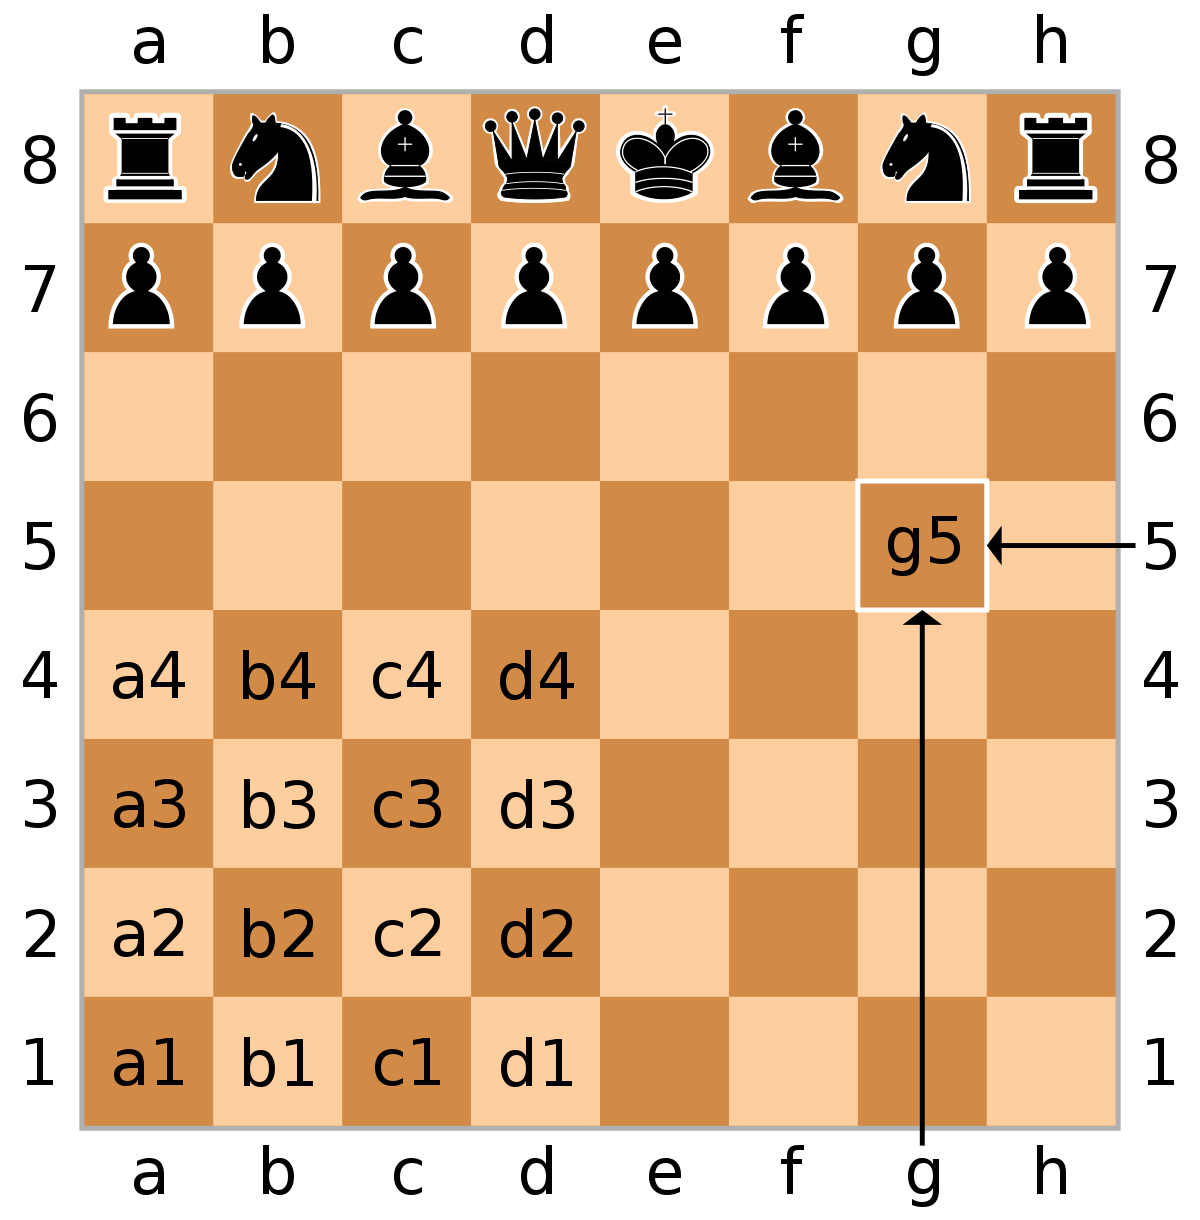
\includegraphics[width=0.4\textwidth]{figures/board-squares.png}
    \caption{Board squares}
    \label{fig:boardSquares}
\end{figure}

Each piece can be identified by a letter (P - pawn, N - knight, B - bishop, R - rook, Q - queen, K - king). Simple SAN moves contain only the destination square, and the letter of piece that moves, if the piece is not a pawn (for example, pawn to c6 is written simply as c6, while knight to c6 is written as Nc6). There are additional rules for moves:
\begin{itemize}
    \item Moves that capture a piece contain the 'x' character right before the destination square (ex: Bxb4)
    \item Castling kingside is written as 'O-O', while queenside castling is written as 'O-O-O'
    \item Moves of pawns to the last rank (promotion moves) contain the equal sign ('=') right after the destination square, followed by the letter of the piece that the pawn promotes to (ex: e8=Q)
    \item If there are more pieces of the same kind that can move to the destination square, the file of the originating square is added right after the piece (ex: Nbc6); if this does not solve the ambiguation, the rank of the originating square is added instead (ex: N8c6), and if neither of these works, both the file and the rank are added (ex: Nb8c6)
    \item If the move checks the opponent's king, a plus sign ('+') is added at the end of the move (ex: Qe7+); if the move checkmates the opponent's king, the octothorpe sign ('\#') is added instead (ex: Qe7\#)
\end{itemize}
\cite{edwards1994standard}

\section{Layers}
\label{sec:ch4sec2}